\documentclass{article} % Especially this!

\usepackage[english]{babel}
\usepackage[utf8]{inputenc}
\usepackage[margin=1.5in]{geometry}
\usepackage{amsmath}
\usepackage{amsthm}
\usepackage{amsfonts}
\usepackage{amssymb}
\usepackage{graphicx}
\usepackage[siunitx]{circuitikz}
\usepackage{tikz}
\usepackage[colorinlistoftodos, color=orange!50]{todonotes}
\usepackage{hyperref}
\usepackage[numbers, square]{natbib}
\usepackage{fancybox}
\usepackage{epsfig}
\usepackage{soul}
\usepackage[framemethod=tikz]{mdframed}
\usepackage[shortlabels]{enumitem}
\usepackage[version=4]{mhchem}
\usepackage{multicol}
\usepackage{graphicx}
\graphicspath{ {./} }

\newcommand{\blah}{blah blah blah \dots}

\setlength{\marginparwidth}{3.4cm}

\newcommand{\summary}[1]{
\begin{mdframed}[nobreak=true]
\begin{minipage}{\textwidth}
\vspace{0.5cm}
\end{minipage}
\end{mdframed}}

\renewcommand*{\thefootnote}{\fnsymbol{footnote}}

\title{
\normalfont \large
\textsc{ASSIGNMENT-4
\vspace{10pt}
\\COL 216, Spring 2021} \\
[10pt] 
\rule{\linewidth}{0.5pt} \\[6pt] 
\Large Memory Request Ordering \\
\rule{\linewidth}{2pt}  \\[10pt]
}
\author{Jitender Kumar Yadav, 2019CS10361
\\Asha Ram Meena, 2019CS10337}
\date{\normalsize \today}
\begin{document}

\maketitle
\section{Problem Statement}
\textbf{Consider the following memory READ address sequence with a DRAM Row size = 1024 bytes: 1000, 2500, 1004, 2504.
\\If we service the requests in the above order, the DRAM will change rows ON EVERY ACCESS, which results in poor performance. Can we do better?
\begin{enumerate}
    \item Sometimes there is an opportunity to change the order in which DRAM requests are serviced. When does this opportunity arise? Assume that the order of instructions and address values of memory instructions cannot be changed.
    \item Design and implement a strategy for efficient ordering of DRAM requests at runtime. Remember   that   the   program’s   semantics   cannot   be   violated   (its   output   cannot change).
\end{enumerate}
Use the same DRAM size/row-size/other architectural assumptions used in the Minor exam. Sample test cases are provided. If you did not handle some of these instruction formats in earlier assignments, please do so now for this assignment.}

\section{Algorithm and Approach}
A MIPS assembly file interpreter for files containing the following instructions was designed in C++: add, sub, mul, beq, bne, slt, j, lw, sw and addi. The memory, register contents, instructions etc. were stored in internal data structures and the program would validate the file for syntax errors and output the hexadecimal register contents and the number of clock cycles and executions. All instructions are red and interpreted in a linear fashion. Any optimizations thus to be made are made on DRAM requests and not on instructions. Thus, a queue was maintained to store DRAM requests issued.
\\In previous assignment, a DRAM model, which is 1024*1024 2D array memory model was implemented. Also, a non-blocking memory was implemented, wherein the following add/sub/mul operations can be carried out while an lw or sw is in progress.
\\In this assignment, another model has been implemented where various DRAM requests can be reordered to minimise the time taken in write-back and copying to buffer.
\begin{itemize}
    \item[$\diamond$] The file containing the instructions is read from the given location and the syntax is checked while storing the instructions in the memory.
    \item[$\diamond$] The instructions are read line by line and the corresponding memory changes are checked and tasks like load, store, addition and subtraction are performed as per need.
    \item[$\diamond$] The data in the 32 registers is stored in an array and so is the auxiliary memory containing $2^{20}$ bits. The registers may be accessed by using MIPS conventions \$s and \$t or by integers 1-32.
    \item[$\diamond$] The operations keep on updating the memory and register contents along side. The register contents are hexadecimal quantities. In case of any wrong memory is accessed by the assembly program, the program returns an error.
    \item[$\diamond$] A queue is maintained where the requests for loading and storing are pushed back to back. The DRAM requests are issued alongside.
    \item[$\diamond$] Once an lw or sw is in progress, among all the DRAM requests, the DRAM requests are chosen such that the execution cycles are less. This is done keeping in mind the fact that the output must not change.
    \item[$\diamond$] When an lw or sw follows some trailing add/addi/mul/sub, the instructions are executed if they aren't affected by the lw or sw.
\end{itemize}

\section{Input and Output}
\subsection{Input Specifications:}
\begin{itemize}
    \item The input is taken on the console while running the executable file a.out.
    \item The first line inputs the name of the MIPS assembly language program as a text file containing the instructions to be executed: add, sub, mul, beq, bne, slt, j, lw, sw, addi. The input format for memory locations is as row\_num(col\_num) where the column number is provided as a register stored value.
    \item The second and third lines input the DRAM timing values row access delay and column access delay, respectively, in cycles.
    \item The fourth line inputs an integer 0 or 1, representing whether to implement the non-blocking mode or DRAM model.
\end{itemize}
\subsection{Output}
\begin{itemize}
    \item The output is a set of printed lines in command line.
    \item At every clock cycle, the clock cycle number and all activity in that cycle is printed, such as:
    \begin{enumerate}
        \item Address of Completed instruction, if any
        \item Modified registers, if any (register number and new value)
        \item Modified memory locations, if any (memory location and new value)
        \item Activity on the DRAM, if any (memory location, row buffer updates)
    \end{enumerate}
    \item After execution completes, the relevant statistics are printed, such as:
    \begin{enumerate}
        \item Total execution time in clock cycles
        \item Number of row buffer updates
        \item The final contents of the registers
        \item The final contents of the memory
    \end{enumerate}
\end{itemize}
\subsection{Sample I/O}
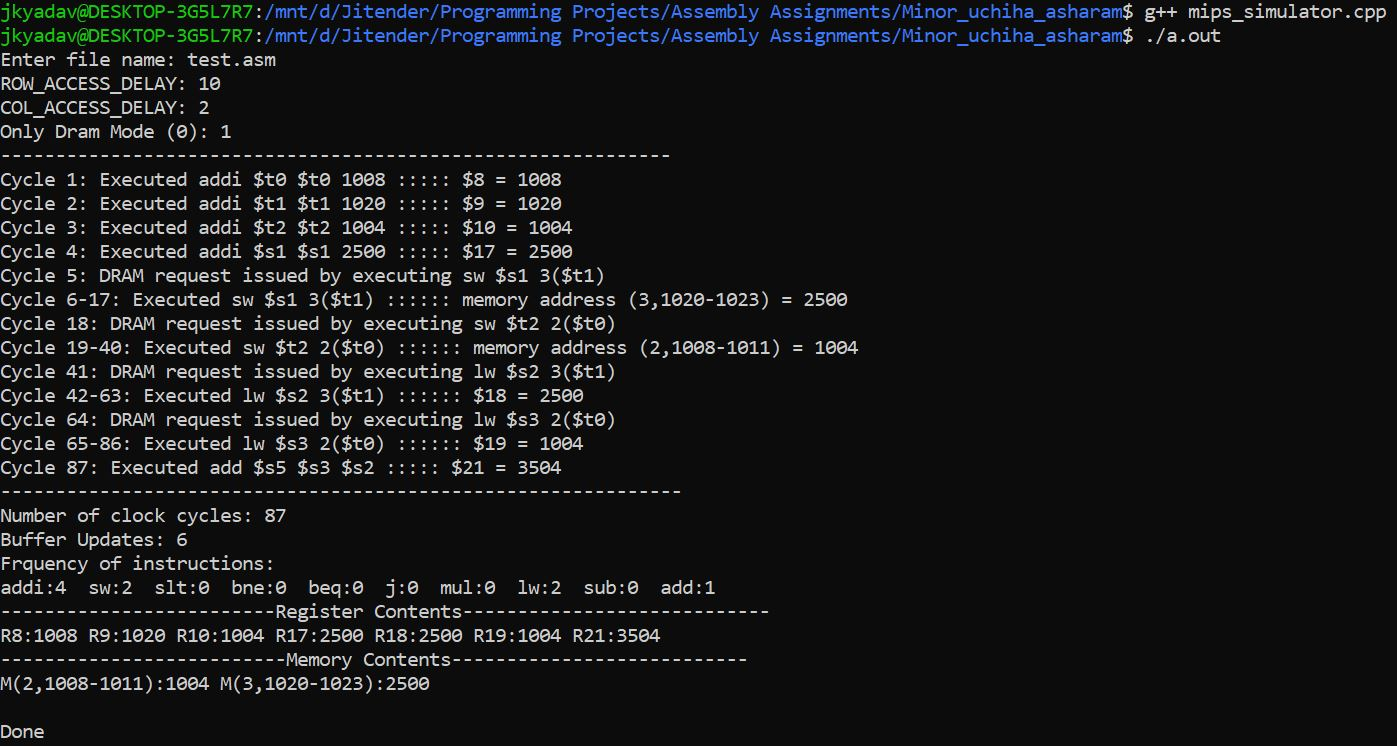
\includegraphics[scale = 0.567]{sampleio_minor.JPG}
\begin{center}
    \textbf{DRAM non-blocking Output}
\end{center}
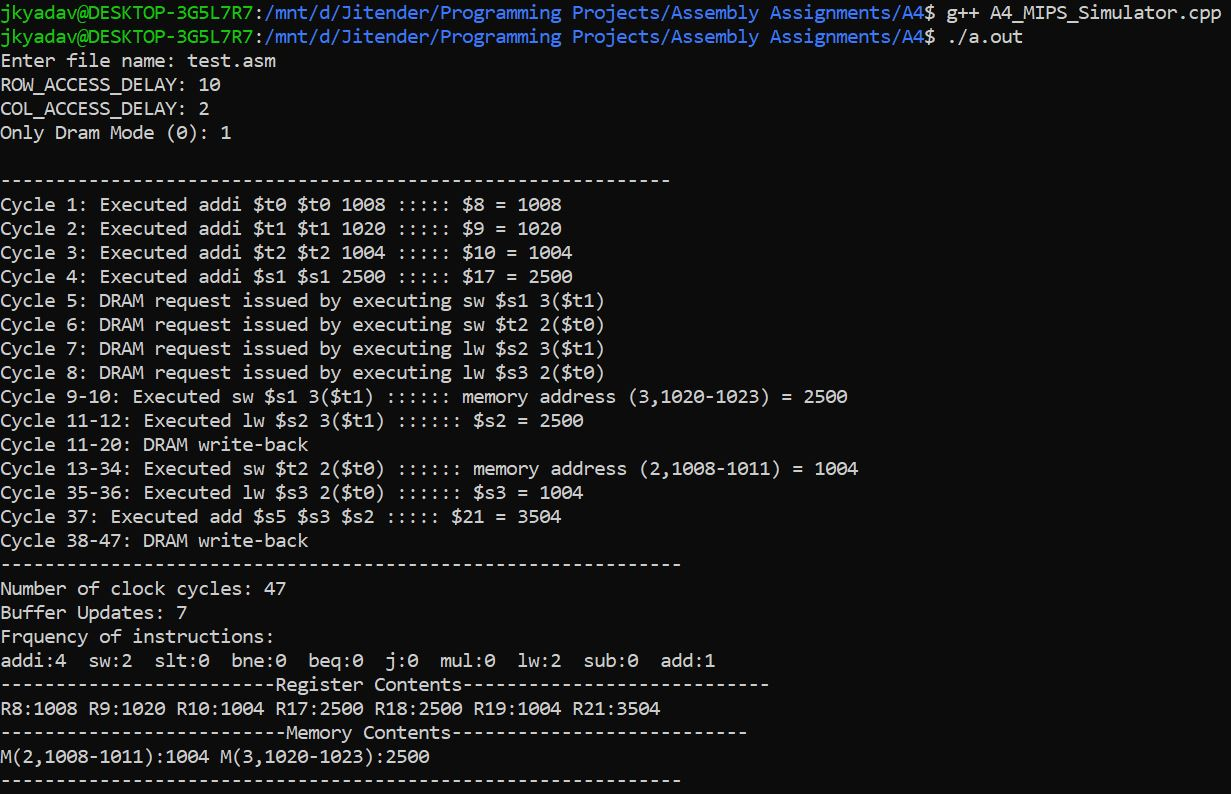
\includegraphics[scale = 0.64]{sampleio_A4.JPG}
\begin{center}
    \textbf{Memory request ordering Output}
\end{center}
The code that was used to compare the output for non-blocking and memory reordering parts is stored in \textbf{\textit{test.asm}} as follows.
\begin{verbatim}
addi $t0 $t0 1008
addi $t1 $t1 1020
addi $t2 $t2 1004
addi $s1 $s1 2500
sw $s1 3($t1)
sw $t2 2($t0)
lw $s2 3($t1)
lw $s3 2($t0)
add $s5 $s3 $s2
\end{verbatim}

\section{Strengths and Weaknesses}
\subsection{Strength}
\begin{enumerate}
    \item The approach can reorder the DRAM requests among a given finite number of DRAM requests, in form of lw and sw commands.
    \item In case an lw or an sw is followed by some add, sub, mul and addi commands, these shall be executed in the cycles along with the ongoing reading and buffer write-back.
    \item This has been achieved with the use of queues to store DRAM requests and reorder them.
\end{enumerate}
\subsection{Weakness}
\begin{enumerate}
    \item It is possible that some add/mul/sub/addi may be blocked and further add and mul may be executed. This has not been done. An add operation which blocks the instruction parsing, stops execution. In other words, let us say some add occurs and can not be executed because it uses some other memory. We may bypass it and execute other instructions. This particular instruction may be executed later.
\end{enumerate}

\section{Testing}
A few test cases were generated to test the Simulator. These have been stored in the directory A4\_TestCases as text files containing the required portion of the asm code. The test cases consider various cases of contiguous lw and sw blocks, such as overlapping memory, overlapping registers, etc.
\\The testing included a large number of test cases which tested all border cases as well as overlapping memory and registers in all contiguous blocks of sw and lw.

\end{document}